\chapter{Experiment Results and Analysis}
\label{chapter:results-and-analysis}
The results of the experiments conducted in this thesis are presented in this chapter. The section \ref{sec:results} presents and describes the results. A more in-depth look at the results is taken in \ref{sec:discussion} where the results are discussed and their significance assessed.

\section{Results}
\label{sec:results}
In this section the results of the three experiments described in~\ref{subsec:measurement-setups} are described. The results of the comparison of the application using the OpenEM dynamic scheduler and the statically scheduled application created with PREESM are given in~\ref{subsec:first-experiment}. The results of the experiment investigating the balance of latency versus throughput are given in~\ref{subsec:second-experiment}. Finally, the results of the third experiment examining the efficiency of increasing the parallelism in the dynamically scheduled application are given in~\ref{subsec:third-experiment}.

\subsection{Comparing Dynamic and Static Scheduling}
\label{subsec:first-experiment}
\FloatBarrier
In the first experiment the bitrates of the two video streams are varied. The latency and throughput of the OpenEM application measurements are summarized in the table \ref{tab:oemthrough2}. The corresponding summaries for the PREESM application are presented in the table \ref{tab:preesmthrough}

The latencies of the two streams of the PREESM application in all measurement setups in the table \ref{tab:preesmthrough} are similar. The largest difference in the latencies is in the case where the Sobel filter filters a CIF stream and the Gauss filter filters a 4CIF stream, where the Gauss latency is 60\% higher than the Sobel latency. Larger differences in the latencies are observed with the OpenEM application with two initial events presented in table \ref{tab:oemthrough2}, where the largest difference in latencies is also measured between the CIF Sobel stream and 4CIF Gauss stream. The Gauss latency in the particular OpenEM measurement is 200\% higher than the Sobel latency. The other OpenEM measurements show larger differences as well compared to PREESM.

\newcommand{\head}[2]{\multicolumn{1}{>{\centering\arraybackslash}p{#1}}{#2}}
\begin{table}
    \begin{center}
        \begin{tabular}{ c c c c c }
            \head{2.6cm}{Sobel latency} & \head{2.6cm}{Gauss latency} &
            \head{1.5cm}{FPS} & \head{2.4cm}{Sobel frame} &
            \head{2.4cm}{Gauss frame} \\ \hline
            3,59 & 10,93 & 256 & CIF & 4CIF \\ \hline
            3,75 & 2,95 & 527 & 4CIF & CIF \\ \hline
            1,42 & 2,80 & 889 & CIF & CIF \\ \hline
            0,32 & 0,71 & 3534 & QCIF & QCIF \\ \hline
        \end{tabular}
        \caption{OpenEM latency and throughput with 2 frames processed simultaneously. The latencies are measured in milliseconds.}
        \label{tab:oemthrough2}
    \end{center}
\end{table}
\begin{table}
    \begin{center}
        \begin{tabular}{ c c c c c }
            \head{2.6cm}{Sobel latency} & \head{2.6cm}{Gauss latency} &
            \head{1.5cm}{FPS} & \head{2.4cm}{Sobel frame} &
            \head{2.4cm}{Gauss frame} \\ \hline
            5,41 & 8,78 & 223 & CIF & 4CIF \\ \hline
            4,65 & 3,54 & 334 & 4CIF & CIF \\ \hline
            2,15 & 2,51 & 668 & CIF & CIF \\ \hline
            0,61 & 0,71 & 2004 & QCIF & QCIF \\ \hline
        \end{tabular}
        \caption{PREESM latency and throughput. The the latencies are measured in milliseconds.}
        \label{tab:preesmthrough}
    \end{center}
\end{table}

The throughput of the application is determined by how much time the application spends processing the streams versus the time spent doing something else. For example the synchronization of all cores before each repetition of the PREESM schedule consumes a lot of CPU cycles as is readily observed from the figure \ref{fig:preesmcif}. The portion of the bars marked as busy corresponds to the cycles spent in the synchronization between the repetitions of the schedule. The percentage of cycles spent in the synchronization varies from 16\% on Core 7 to 45\% on Core 0. The OpenEM dynamic scheduler seems to spread out the work more evenly in this case where the total overhead cycles are approximately 60\% for all cores. The core utilization per function is presented in figure \ref{fig:oem8corefunc}. Most of the overhead cycles in the OpenEM application are spent waiting for more frames for processing.

\begin{figure}
    \centering
    \begin{subfigure}[t]{0.49\textwidth}
        \centering
        \includegraphics[width=0.99\linewidth]{images/preesm_cifcif.eps}
        \caption{PREESM}
        \label{fig:preesmcif}
    \end{subfigure}
    \begin{subfigure}[t]{0.49\textwidth}
        \centering
        \includegraphics[width=0.99\linewidth]{images/openem_cifcif_2initial_func.eps}
        \caption{OpenEM}
        \label{fig:oem8corefunc}
    \end{subfigure}
    \caption{In the PREESM graph the busy portion of the bars correspond to the cycles spent synchronizing the cores between the repetitions of the block schedule. The overhead corresponds to cycles spent outside the measured functions and the synchronization. In the OpenEM application the overhead cycles are the cycles spent outside the compared functions.}
\end{figure}

The overhead portions in the figures \ref{fig:preesmcif} and \ref{fig:oem8corefunc} contain all of the data copying from buffer to buffer outside the measured functions, but they also contain different amounts of cycles spent in communications between the cores. The measured functions are the functions, which are explicitly called in the PREESM actor model. Other functions not included in the measured functions contain runtime specific communication and some copying of buffers.

\FloatBarrier
\subsection[Investigating the Balance of Latency and Throughput]{Investigating the Balance of Latency\\and Throughput}
\label{subsec:second-experiment}
\FloatBarrier
In this set of measurements the OpenEM application is configured to process different numbers of frames simultaneously. The PREESM latencies in the table \ref{tab:preesmthrough} are consistently smaller than the latencies of the throughput optimized OpenEM application in the table \ref{tab:oemthrough}. The throughput optimized application is processing 16 frames simultaneously. The throughput of the OpenEM application is almost doubled compared to the configuration presented in \ref{tab:oemthrough2} where two frames processed simultaneously.

The effect of increasing the number of simultaneous frames was further examined by measuring the application with two CIF streams using 2 to 24 initial events. The results of the measurements are presented in table \ref{tab:oeminitialframes}. The throughput is increased when the number of frames processed simultaneously increases. This behavior is visualized in figures \ref{fig:oeminitialframesfps} and \ref{fig:oeminitialframeslat}. The throughput grows rapidly up to 8 simultaneous frames, after which the growth slows down. The latencies grow with each added frame steadily.

\begin{table}
    \begin{center}
        \begin{tabular}{ c c c c c }
            \head{2.6cm}{Sobel latency} & \head{2.6cm}{Gauss latency} &
            \head{1.5cm}{FPS} & \head{2.4cm}{Sobel frame} &
            \head{2.4cm}{Gauss frame} \\ \hline
            15,82 & 22,85 & 599 & CIF & 4CIF \\ \hline
            4,85 & 3,67 & 895 & 4CIF & CIF \\ \hline
            4,91 & 5,96 & 1955 & CIF & CIF \\ \hline
            1,33 & 1,62 & 7819 & QCIF & QCIF \\ \hline
        \end{tabular}
        \caption{OpenEM latency and throughput with 16 frames processed simultaneously. The latencies are measured in milliseconds.}
        \label{tab:oemthrough}
    \end{center}
\end{table}

\begin{figure}
    \centering
    \begin{subfigure}[t]{0.49\textwidth}
        \centering
        \includegraphics[width=0.99\linewidth]{images/simultaneous_frames_fps.eps}
        \caption{FPS as a function of simultaneous frames.}
        \label{fig:oeminitialframesfps}
    \end{subfigure}
    \begin{subfigure}[t]{0.49\textwidth}
        \centering
        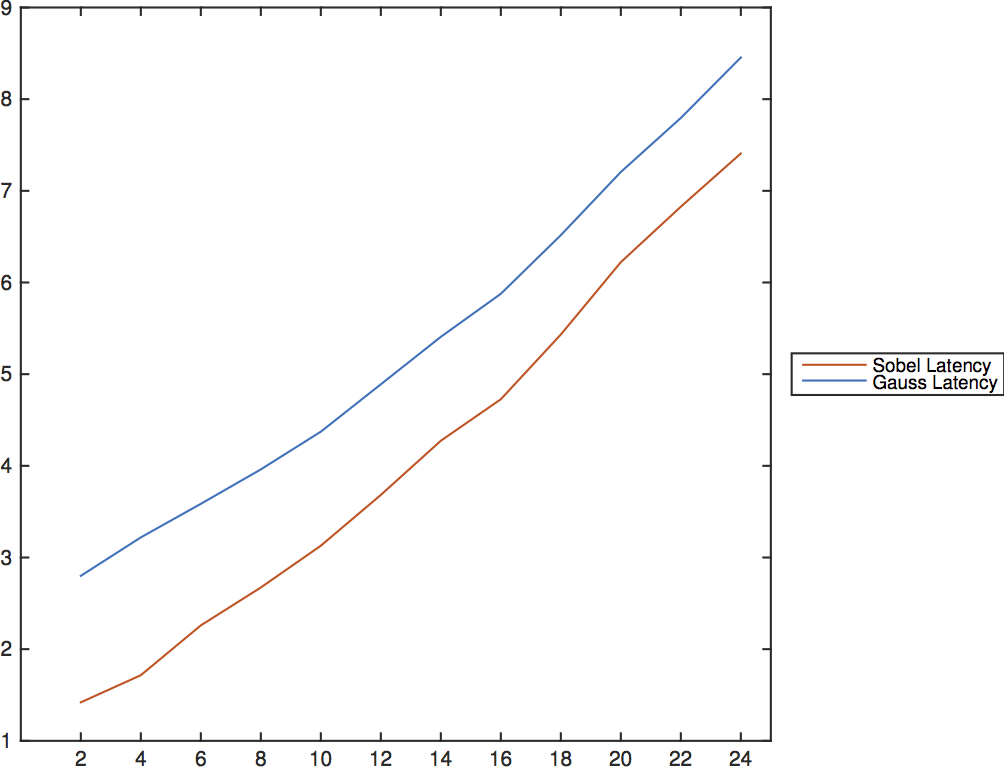
\includegraphics[width=0.99\linewidth]{images/simultaneous_frames_latency-eps-converted-to-png.png}
        \caption{Latencies as functions of simultaneous frames. The latencies are measured in milliseconds.}
        \label{fig:oeminitialframeslat}
    \end{subfigure}
    \caption{The effect of increasing the number of frames processed simultaneously is presented in the figures. The throughput increases rapidly up to 8 simultaneous frames after which the growth slows down. The latency grows more steadily across all measured setups.}
\end{figure}
\begin{table}
    \begin{center}
        \begin{tabular}{ c c c c }
            \head{2.6cm}{Sobel latency} & \head{2.6cm}{Gauss latency} &
            \head{1.5cm}{FPS} & \head{3.3cm}{Simultaneous Frames} \\
            \hline
            1,42  &  2,80  &  889   &  2 \\ \hline
            1,72  &  3,22  &  1371  &  4 \\ \hline
            2,26  &  3,59  &  1655  &  6 \\ \hline
            2,67  &  3,96  &  1825  &  8 \\ \hline
            3,13  &  4,37  &  1880  &  10 \\ \hline
            3,68  &  4,89  &  1921  &  12 \\ \hline
            4,27  &  5,40  &  1940  &  14 \\ \hline
            4,73  &  5,88  &  1958  &  16 \\ \hline
            5,43  &  6,52  &  1976  &  18 \\ \hline
            6,22  &  7,21  &  1983  &  20 \\ \hline
            6,83  &  7,80  &  1981  &  22 \\ \hline
            7,41  &  8,45  &  1992  &  24 \\ \hline
        \end{tabular}
        \caption{OpenEM measurements with different numbers of frames in processed simultaneously.}
        \label{tab:oeminitialframes}
    \end{center}
\end{table}

\FloatBarrier
\subsection{Examining the Efficiency of Parallel Scheduling}
\label{subsec:third-experiment}
\FloatBarrier
In the third experiment the number of cores available for the OpenEM application was varied. Both filters were processing CIF streams. The measurements were repeated using one to eight cores. The resulting latencies and throughputs are presented in the table \ref{tab:oemcoremasks}. The increase of the throughput of the OpenEM application is presented in figure \ref{fig:fpsvcores}. The actual FPS measured with eight cores is approximately 90\% of the linear growth calculated from the FPS using a single core.
\begin{table}
    \begin{center}
        \begin{tabular}{ c c c c }
            \head{2.6cm}{Sobel latency} & \head{2.6cm}{Gauss latency} &
            \head{1.5cm}{FPS} & \head{2.0cm}{No of cores} \\
            \hline
            57,05 & 57,11 & 263 & 1 \\ \hline
            22,59 & 23,15 & 510 & 2 \\ \hline
            15,09 & 15,84 & 768 & 3 \\ \hline
            10,91 & 11,85 & 1014 & 4 \\ \hline
            8,41 & 9,53 & 1268 & 5 \\ \hline
            7,05 & 8,07 & 1500 & 6 \\ \hline
            5,74 & 6,83 & 1731 & 7 \\ \hline
            4,91 & 5,96 & 1955 & 8 \\ \hline
        \end{tabular}
        \caption{OpenEM measurements with number of cores varied}
        \label{tab:oemcoremasks}
    \end{center}
\end{table}
\begin{figure}
    \begin{center}
        \includegraphics[width=0.7\textwidth]{images/coremask_fps.eps}
        \caption{FPS increase as the function of cores vs. linear growth}
        \label{fig:fpsvcores}
    \end{center}
\end{figure}
\FloatBarrier

\section{Discussion}
\label{sec:discussion}
Three experiments were conducted to understand the performance of Open Event Machine based multi-core DSP applications in stream processing. The studied stream processing application was implemented with OpenEM and a comparable application was implemented using PREESM. The performance of the applications as a part of a stream processing system was not studied. Therefore, IO was omitted from the stream processing task that both of the applications implemented. The experiments focused on understanding the performance of the OpenEM scheduler in handling stream processing tasks.

In this section the results of the three conducted experiments are discussed. First, the discoveries made from the experiments are described in \ref{subsec:discoveries}. Second, the possible directions of future work are discussed in \ref{subsec:future-work}. Finally, the challenges faced conducting the experiments are explained in \ref{subsec:challenges}

\subsection{Discoveries}
\label{subsec:discoveries}
\FloatBarrier
The first experiment where the throughput and latency of OpenEM based application were compared to those of the statically scheduled application showed that the runtime systems are roughly comparable. The statically scheduled application created with PREESM potentially had the advantage here, since with static schedule no cycles are wasted at any point in the execution in deciding which actor to execute next on which core. OpenEM achieved very similar latencies with the dynamic scheduler. This suggests that the OpenEM scheduler utilizes the hardware resources efficiently and causes relatively small overhead.

The PREESM authors state that PREESM is a prototyping tool~\cite{preesm}, which suggests that it does not necessarily aim to create latency or throughput optimized applications. The Gantt chart in figure~\ref{fig:preesm_gantt} suggests that manually optimizing the schedule, a lower latency and higher throughput could be achievable. This is supported by the core utilization graph in figure~\ref{fig:preesmcif} where a large portion of the execution time is spent waiting for other cores. Nevertheless, the OpenEM scheduling performance can be considered good as it roughly matches the statically generated schedule.

In the second experiment the balance of latency versus throughput with the OpenEM scheduler was investigated. The experiment where the number of simultaneously processed frames was varied suggested that by configuring the application the balance between throughput and latency can be controlled. The adjustability of the scheduler is a useful feature to have in real applications, as the throughput can be increased for tasks, which are less latency sensitive without modifying the program code. The extent of control the application designer has depends on the complexity of the application. The application measured in the experiments was simple and it is possible that the results overemphasize the adaptivity compared to more complex applications.

The third experiment was conducted to understand the performance improvement gained from making more processing units available for the runtime. The FPS improvement from one to eight cores is close to 90\% of linear improvement. This means that the sequential portion of the application was small and the scheduler was able to utilize the increased parallelism efficiently.

Since two frames are processed simultaneously the execution of the serial part of the program performed in the read and merge execution objects is interleaved with the execution of the filter execution object of the other frame. This behavior seems to yield a large latency decrease from execution on one core to execution on two cores. Unfortunately this complicates the analysis, since the proportion of the serial and parallel parts of the program is ambiguous. This complication prevents useful comparisons with the theoretical improvement defined by Amdahl's law~\cite{amdahl1967validity}.

The result of the parallel scheduling experiment was not surprising but it is reassuring of the OpenEM scheduler performance. As the total number of events in circulation was quite small compared to the example applications provided with the TI OpenEM distribution \cite{openemuser}, the scheduler should have no trouble keeping up with the pace of the application even with eight cores.

\begin{figure}
    \centering
    \begin{subfigure}[t]{0.49\textwidth}
        \centering
        \includegraphics[width=0.99\linewidth]{images/openem_cifcif_8cores_eo.eps}
        \caption{Sobel CIF, Gauss CIF}
        \label{fig:oem8coreeo}
    \end{subfigure}
    \begin{subfigure}[t]{0.49\textwidth}
        \centering
        \includegraphics[width=0.99\linewidth]{images/openem_sobel4cif_gausscif_eo.eps}
        \caption{Sobel 4CIF, Gauss Cif}
        \label{fig:oem8coreeosobel4cif}
    \end{subfigure}
    \caption{The bottleneck forming due to the atomic read operation can be observed by comparing the core utilization when both of the streams are at CIF resolution to the case where Sobel resolution is increased to 4CIF. In these graphs the application is processing 16 simultaneous events.}
\end{figure}

The throughput optimized application processing 16 events simultaneously exhibits formation of a bottleneck in the atomic execution object. In the table \ref{tab:oemthrough} an improvement of latencies is observed when the workload is made heavier by moving 4CIF stream from Gauss filter to the Sobel filter while the other stream is kept at CIF resolution.

The probable cause of the improvement of the latencies when the workload is made heavier by increasing the Sobel stream resolution is the reduced interleaving of the processing of the subsequent frames. The reduction in the interleaving is caused by the read execution object, which is only connected to an atomic queue. When the frame size of the Sobel stream is increased the read EO starts limiting the throughput of the application. Fewer frames are processed in parallel, which decreases the time from reading each individual frame to the completion of that frame.

The formation of the bottleneck can be observed by comparing the core utilization in the figure \ref{fig:oem8coreeo} to the core utilization in the figure \ref{fig:oem8coreeosobel4cif} where seven cores need to wait for the read operations on the Core 2 and the overall overhead is increased. The other cores do not receive any events from the OpenEM scheduler while waiting.

\begin{figure}
    \begin{center}
        \includegraphics[width=0.49\textwidth]{images/openem_sobelcif_gauss4cif_eo.eps}
        \caption{OpenEM cycles spent per execution object for CIF Sobel frames
        and 4CIF Gauss frames}
        \label{fig:oem8coreeogauss4cif}
    \end{center}
\end{figure}

When the Gauss stream is increased to 4CIF and the Sobel stream is kept at CIF the bottleneck does not form. This is likely because computing the Gaussian filter for the 4CIF frames is consuming approximately 80\% of the cycles on all cores. In this case the read EO only consumes approximately 5\% to 13\% of the cycles on all cores. Compared to the case of two CIF streams, the latencies in this case are increased by factors of approximately 3 and 4 for Sobel and Gauss correspondingly. The resulting core utilization graph is presented in figure \ref{fig:oem8coreeogauss4cif}.
\FloatBarrier

\subsection{Future Work}
\label{subsec:future-work}
In this thesis the use of OpenEM to provide task management and scheduling in a stream processing application was investigated. The results suggest that OpenEM scales well to the needs of a simple stream processing application and it simplifies the implementation of a multi-core application on the DSP platform without operating system.

The workload studied in this thesis was simple and lacked dynamic nature of processing graphs common to stream processing applications. To better understand the performance of OpenEM, two future research approaches could be taken. First, studying the performance of OpenEM scheduler with another artificial workload application could still strengthen the case for using OpenEM as the runtime for stream processing. Instead of a simple, linear processing graph like the one used in the experiments of this thesis, a more dynamic graph with optional processing paths could be studied. Studying this kind of graph would show if the scheduler is capable of hitting the latency and throughput constraints of the application consistently under varying load. Second, a more complex application could be constructed and measured. For example implementing an MPEG decoder using OpenEM as the runtime system would provide a more complete view to the dynamic performance of OpenEM. An MPEG decoder would be an interesting workload because it has been used as something of a standard benchmark in dataflow literature and thus there exists many implementations based on different technologies. Having points of comparison for the workload would help put the performance in broader context.

The idea of using DSPs for stream processing has been researched to some extent but the idea has not made it to the mainstream of computing industry. To make the case for DSPs as stream processors, a thorough benchmark should be created that would compare the streaming performance versus energy consumed for similar stream processing applications implemented with DSPs, GPUs, and CPUs. Making such comparison is not trivial, since to the author's knowledge there does not exist a single widely accepted measure of streaming performance. The question is complicated further by the need for measuring the energy consumption, which itself is a complex task.

Before conducting such research, three problems would have to be solved. First, selection of the measured variables. Comparing floating point operations per second per Joule between the platforms would be the simple solution, but FLOPS is not necessarily good measurement for streaming performance. For example, for video stream, frames per second and latency would provide a better understanding of the streaming performance than FLOPS. Second, accounting of the energy consumption fairly with all measured processing units is not trivial, since they are commonly installed in different forms of devices. CPUs are installed in sockets on motherboards, GPUs are installed on PCI cards or increasingly as part of integrated chips, and DSPs are installed in various devices including PCI cards. Comparing the vendor provided energy specifications is one way to deal with this problem, but it might miss how the devices are actually deployed. Third, the workload would have to be implemented in different patterns for each of the platforms making use of the strengths of each platform equally.

Two papers conduct comparisons that partially answer the questions above, but do not actually provide the complete comparison between the processors. Stotzer et al. conduct an experiment in~\cite{stotzer2013openmp} where a comparison between the different processing units is conducted in the context of OpenMP, but the comparison does not include energy measurements. The performance of FPGAs and GPUs in processing what the author calls ``sliding-window applications'' is compared in terms of Joules per frame in~\cite{fowers2012performance}. The ``sliding-window applications'' consist of applying convolutions on frames of data in the stream, similar to how the workload in this thesis computes.

\subsection{Challenges}
\label{subsec:challenges}
Analysing the performance of OpenEM based stream processing applications is a broad task, requiring the use of many distinct technologies. First, a suitable workload, which is representative of stream processing tasks had to be designed. Next, two versions of the workload application had to be implemented, one for the evaluation of OpenEM and the other to provide a point of comparison. In order to get usable data from the applications, they had to be instrumented and the measurement data analysed. Most of the work required was straightforward but some complications were faced with the tools.

The baseline application was implemented using PREESM. PREESM generates static schedules for the application from provided the dataflow graph and the source code. To get specific points of comparison for each of the measurement setups working with the PREESM automatic code generation was complicated. The tool would create different schedules on each iteration and thus yield applications with dissimilar core usage between the measurement setups.

Texas Instruments OpenEM version 1.0.0.2 that was used for the implementation of the OpenEM workload has some unimplemented features. Most of the unimplemented features were documented and did not cause unnecessary work. However, the implementation of Queue Groups did not work as expected. Creation of multiple queue groups did not work as specified in the documentation, and was left unexplored after multiple trials at working with them.

The documentation of the Texas Instruments implementation of OpenEM was lacking. The documentation provided with the source code was incomplete and included a sketchy version of the OpenEM white paper~\cite{moerman2014open}, which was the most important source for understanding the use of hardware acceleration in the runtime. The documentation also lacked details for the initialization layer without which the initialization of the hardware components would have been difficult. The initialization code was provided as a part of a scarcely documented example application.
